\documentclass{standalone}

\usepackage{tikz}
\usetikzlibrary{positioning}
\usetikzlibrary{calc}





\begin{document}

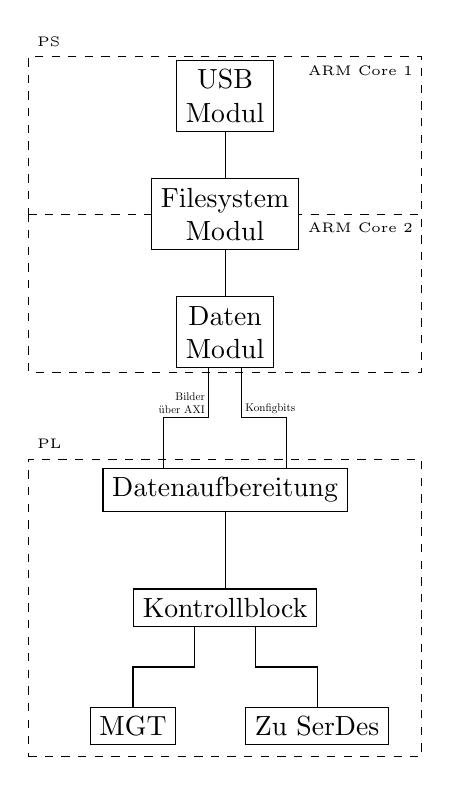
\begin{tikzpicture}
    %core 1
    \node[yshift=-0.5cm, draw, dashed, minimum height=2cm, minimum width=5cm] at (0,0) (core1) {};
    \node[anchor=north east] at (core1.north east) {\tiny ARM Core 1};
    %core 2
    \node[yshift=0.5cm, minimum height=2cm, minimum width=5cm] at (0,-3) (core2) {};
    \draw[dashed] ([xshift=0.5\pgflinewidth]core2.north west) -- ([xshift=0.5\pgflinewidth]core2.south west) -- ([xshift=-0.5\pgflinewidth]core2.south east) -- ([xshift=-0.5\pgflinewidth]core2.north east);
    \node[anchor=north east] at (core2.north east) {\tiny ARM Core 2};
    %PS
    %\node[draw, dashed, minimum height=4.5cm, minimum width=6cm] at (0,-1.5) (ps) {};
    \node[anchor=south west] at (core1.north west) {\tiny PS};
    %USB
    \node[draw, align=center] at (0, 0) (usb) {USB\\Modul};
    %Filesystem
    \node[fill=white, draw, align=center] at (0, -1.5) (file) {Filesystem\\Modul};
    %Datenmodul
    \node[draw, align=center] at (0, -3) (daten) {Daten\\Modul};
    %Datenaufbereitung
    \node[draw] at (0,-5) (auf) {Datenaufbereitung};
    %Kontrollblock
    \node[draw] at (0,-6.5) (kontroll) {Kontrollblock};
    %MGT
    \node[draw] at (0,-8 -| kontroll.west) (mgt) {MGT};
    %Zu SerDes
    \node[draw] at (0,-8 -| kontroll.east) (serdes) {Zu SerDes};
    %PL
    \path let \p{1} = ($(auf.north)-(mgt.south)$) in node[draw, dashed, minimum width=5cm, minimum height=\y1+0.25cm] at (kontroll) (pl) {};
    \node[anchor=south west] at (pl.north west) {\tiny PL};





    %USB zu Filesystem
    \draw (usb) -- (file);
    %Filesystem zu Daten
    \draw (file) -- (daten);
    %Datenmodul - Datenaufbereitung AXI
    \draw ($(daten.south west)!1/3!(daten.south east)$) |- ({$(daten.south)!1/2!(auf.north)$} -| {$(auf.south west)!1/4!(auf.south east)$}) node[pos=0.5, anchor=south east, align=right, scale=0.4] {Bilder\\über AXI} -- ($(auf.north west)!1/4!(auf.north east)$);
    %Datenmodul - Datenaufbereitung Konfigbits
    \draw ($(daten.south west)!2/3!(daten.south east)$) |- ({$(daten.south)!1/2!(auf.north)$} -| {$(auf.south west)!3/4!(auf.south east)$}) node[pos=0.5, anchor=south west, scale=0.4] {Konfigbits} -- ($(auf.north west)!3/4!(auf.north east)$);
    %Datenaufbereitung - kontrollblock
    \draw (auf) -- (kontroll);
    %Kontrollblock - MGT
    \draw ($(kontroll.south west)!1/3!(kontroll.south east)$) |- ({$(kontroll.south)!1/2!(mgt.north)$} -| {mgt})  -- (mgt);
    %Kontrollblock - SerDes
    \draw ($(kontroll.south west)!2/3!(kontroll.south east)$) |- ({$(kontroll.south)!1/2!(serdes.north)$} -| {serdes})  -- (serdes);

\end{tikzpicture}

\end{document}